% 발표 자료 (한국어) — FIDE 규칙 하 체스 게임의 최대 길이는 17,697 플라이.
%
% 빌드:  tectonic slides-ko.tex          (슬라이드)
%        tectonic slides-ko-notes.tex    (발표 대본)
% 그림·스크린샷 재생성:  uv run --with cairosvg --with playwright --with pymupdf \
%                          python make_assets.py
% 폰트: Noto Sans KR 필요 — README.md 참고.
%
% 서술 방식: 슬라이드는 정의·정리·증명을 본문과 같은 번호로 진술하고 그림을
% 붙인다. 말로 풀 내용은 \note{}에 있으며 slides-ko-notes.tex 가 그것만
% 뽑아 대본 PDF를 만든다. 정리 번호는 자동 계수가 아니라 손으로 적는다 ---
% 슬라이드 순서가 아니라 main.tex 와 일치해야 하기 때문이다.
\documentclass[aspectratio=169,10pt]{beamer}
\usepackage{longchess}
\usepackage{xeCJK}
\xeCJKsetup{CJKspace=true}
% 숫자·라틴문자와 한글 사이의 자동 글루를 끈다: "2026년 8월"이
% "2026 년 8 월"로 벌어지는 것을 막는다. 띄어쓰기는 원고에서 직접 준다.
\xeCJKsetup{CJKecglue={}}
\setCJKmainfont{Noto Sans KR}
\setCJKsansfont{Noto Sans KR}

\newcommand{\B}{\mathsf{B}}
\newcommand{\W}{\mathsf{W}}

% ---- 그림 안에 들어가는 낱말들 (lcfigures.sty 가 쓰는 어휘) ----------------
% 본문이 영어 용어를 그대로 쓰는 것(critical move 등)은 그대로 둔다.
\renewcommand{\lcsPly}{플라이}
\renewcommand{\lcsClock}{하프무브 클록}
\renewcommand{\lcsCritical}{critical move}
\renewcommand{\lcsQuiet}{quiet 플라이}
\renewcommand{\lcsGameEnds}{게임 종료}
\renewcommand{\lcsSegment}{세그먼트}
\renewcommand{\lcsSegments}{세그먼트}
\renewcommand{\lcsSwitch}{색 전환}
\renewcommand{\lcsSwitches}{색 전환}
\renewcommand{\lcsWhite}{백}
\renewcommand{\lcsBlack}{흑}
\renewcommand{\lcsPawnMoves}{폰 이동}
\renewcommand{\lcsCaptures}{포획}
\renewcommand{\lcsOverlaps}{겹침}
\renewcommand{\lcsClosing}{종결 세그먼트}
\renewcommand{\lcsResolved}{resolved 파일 수 $f$}
\renewcommand{\lcsPawn}{폰}
\renewcommand{\lcsPawns}{폰}
\renewcommand{\lcsHomeRank}{홈 랭크}
\renewcommand{\lcsPromotes}{승격}
\renewcommand{\lcsStuck}{막힘}
\renewcommand{\lcsCaptured}{잡힘}
\renewcommand{\lcsNoPawnMove}{폰 이동 0}
\renewcommand{\lcsImpossible}{전부 infeasible}
\renewcommand{\lcsSurvives}{유일한 생존자}
\renewcommand{\lcsFirstPhase}{첫 구간}
\renewcommand{\lcsMiddleBlock}{가운데 블록}
\renewcommand{\lcsSameColour}{양 끝 같은 색}
\renewcommand{\lcsDiffColour}{양 끝 다른 색}
\renewcommand{\lcsEven}{짝수 길이}
\renewcommand{\lcsOdd}{홀수 길이}
\renewcommand{\lcsTypicalGame}{보통의 대국}
\renewcommand{\lcsLongestGame}{최장 게임}
\renewcommand{\lcsPlies}{플라이}
\renewcommand{\lcsDeadPos}{dead position}
\renewcommand{\lcsMate}{체크메이트}
\renewcommand{\lcsBudget}{손으로 증명}
\renewcommand{\lcsSpent}{사용}
\renewcommand{\lcsTarget}{목표}
\renewcommand{\lcsWhyOne}{한 색만 폰을 움직임}
\renewcommand{\lcsWhyTwo}{희생자 14개가 못 움직임}
\renewcommand{\lcsWhyThree}{홈 랭크가 4수로 묶음}
\renewcommand{\lcsVerifier}{독립 검증기}
\renewcommand{\lcsTrace}{플라이별 trace}
\renewcommand{\lcsVerdict}{판정}
\renewcommand{\lcsChecker}{산술 검사기}
\renewcommand{\lcsAgree}{판정 일치}
\renewcommand{\lcsCritOfX}{$X$의 모든 critical move}
\renewcommand{\lcsCritOfY}{$Y$의 모든 critical move}
\renewcommand{\lcsTwoBlockLoss}{$Y$-폰 $\ge7$개가 잡혀 폰 이동 $0$}
\renewcommand{\lcsThreeBlockNeed}{$X$-폰 $\ge7$개가 잡힘 $\Rightarrow$
  폰 이동 $6\times7$이 전부 첫 구간 안에}
\renewcommand{\lcsThreeBlockCap}{그런데 홈 랭크가 폰당 $4$로 묶는다}
\renewcommand{\lcsProof}{증명}
\renewcommand{\lcsSketch}{증명 (개요)}
\renewcommand{\lcsRepetition}{동일 포지션 5회 반복}
\renewcommand{\lcsSamePos}{같은 포지션이 다섯 번}
\renewcommand{\lcsSeventyFive}{양측 각 75수}
\renewcommand{\lcsClockHits}{클록이 150에 도달}
\renewcommand{\lcsDeadTitle}{dead position}
\renewcommand{\lcsNoMate}{어떤 수순으로도 메이트 불가}
\renewcommand{\lcsOnlyPawn}{폰 이동만}
\renewcommand{\lcsOnlyCap}{포획만}
\renewcommand{\lcsBoth}{둘 다}
\renewcommand{\lcsCritMoves}{critical move 총수}
\renewcommand{\lcsSixRanks}{승격까지 여섯 랭크}
\renewcommand{\lcsSixteen}{폰 $16$개 $\times$ $6$수}
\renewcommand{\lcsGamesWorth}{보통의 대국을 이어붙인 길이}

% ---- 발표 구성 -------------------------------------------------------------
\def\lcmapn{7}
\def\lcmapnames{{0.~서론},{I.~규칙},{II.~계수},{III.~전환},%
  {IV.~탐색},{V.~검증},{VI.~의의}}

% Short forms feed Madrid's footline: author (institute) | title | date.
\title[체스 게임의 최대 길이]{체스 게임의 최대 길이는 17{,}697 플라이다}
\subtitle{The maximum length of a chess game under the FIDE Laws\\
  is 17{,}697 plies}
\author[임준엽]{임준엽}
\institute[공주대]{공주대학교 응용수학과}
\date[2026.8]{2026년 8월}

\begin{document}

\lctitleframe
\note{본 발표에서 증명할 명제는 하나입니다. 체스 게임의 최대 길이는 정확히
17{,}697 플라이다. 값 자체는 2015년부터 알려져 있었고, 없던 것은 그보다 긴
게임이 존재하지 않는다는 증명입니다.}

% =========================================================== 0. 서론
\lcpart{0}{서론}{알려진 값, 없던 증명}

\begin{frame}{문제의 출처}
  \centering
  \vspace{0.3cm}
  \begin{columns}[c]
    \begin{column}{0.36\textwidth}\centering
      \lcshot{5.0cm}{assets/shot-yt-video.jpg}{[유튜브 썸네일]}\\[3pt]
      \lccap{유튜버 \textbf{잉체스}(증강체스 개발자)}
    \end{column}
    \begin{column}{0.05\textwidth}\centering
      {\Large\color{lcmid}$\rightarrow$}
    \end{column}
    \begin{column}{0.36\textwidth}\centering
      \lcshot{5.0cm}{assets/shot-labelle.png}{[wismuth.com 캡처]}\\[3pt]
      \lccap{F.~Labelle, \emph{The longest possible chess game}, 2015}
    \end{column}
  \end{columns}
  \par\vspace{0.55cm}
  \lcquote{``\emph{I believe} that the length of the longest possible
    chess game is $8848.5$ moves.''}{Labelle 2015}
  \note{출발점은 유튜버 잉체스---변형체스 웹게임 증강체스를 만든 분입니다---의
  영상이었습니다. ``이론상 가장 긴 체스 게임''.

  그 영상의 설명란이 François Labelle의 페이지로 이어집니다. 그 페이지에
  사실상 전부가 있습니다. 118개의 delay ply, 색 전환 세 번짜리 스케줄, 완전한
  기보.

  그런데 결론 문장이 ``I believe''입니다. 값은 알려져 있었지만 증명은 없었던
  겁니다. 본 발표는 그 증명입니다.}
\end{frame}

\begin{frame}{발표 구성}
  \centering
  \lcmap{0}
  \par\vspace{0.85cm}
  {\small
  \begin{tabular}{@{}ll@{}}
    \textbf{I--III} & 상한의 증명 --- 손으로 검산 가능한 조합론 \\[4pt]
    \textbf{IV--V}  & 계산 --- 선행 탐색과 검증 \\[4pt]
    \textbf{VI}     & 결과의 의의 \\
  \end{tabular}}
  \par\vspace{0.75cm}
  \lcquote{$L \;\le\; 150 \cdot 118 - 3 \;=\; \mathbf{17{,}697}$}{}
  \note{발표는 일곱 부분이고, 성격이 다릅니다.

  I부터 III까지는 순수하게 수학이며 컴퓨터가 등장하지 않습니다. IV와 V는
  전부 계산 이야기입니다---선행 탐색과 검증. VI는 의의입니다.

  도착점은 저 식 하나입니다. 세그먼트 150개짜리가 118개, 빼기 3. 저 3이
  이 논문의 핵심입니다.

  정리 번호는 본문 번호를 그대로 씁니다. 나중에 논문에서 찾으실 수 있도록.}
\end{frame}

% =========================================================== I. 규칙
\lcpart{I}{규칙}{2014년, 체스가 유한해지다}

\begin{frame}{자동 종료 규칙 --- 2014년 7월 1일 발효}
  \centering
  \lcmap{1}
  \par\vspace{0.45cm}
  \figrules
  \par\vspace{0.35cm}
  {\small 2014년 이전: 3회 반복·50수 무승부는 \emph{선언}해야 성립 ---
   협력하는 두 플레이어는 영원히 둘 수 있다 (Euwe 1929, Thue--Morse).}
  \note{2014년 이전에는 이 질문에 유한한 답이 없었습니다. 3회 반복도 50수
  규칙도 선언해야 성립했으니, 협력하는 두 사람은 영원히 둘 수 있었습니다.
  Euwe가 1929년에 Thue--Morse 수열을 재발견하며 보인 고전적 사실입니다.

  2014년 7월 1일부터 FIDE 규칙은 게임을 자동으로 종료합니다. 선언이 필요
  없습니다.

  첫째, 같은 포지션이 다섯 번 나오면 종료. 둘째, 양측이 각각 75수 동안 폰
  이동도 포획도 없으면 종료---클록이 150에 닿는 순간입니다. 셋째는 원래
  있던 dead position 조항이고, 킹 둘만 남은 자리가 그 전형입니다.

  이 규칙에는 실효성이 있습니다. 7-piece 테이블베이스에는 500수가 넘는 강제
  메이트가 있는데, 두 번째 규칙이 그것을 전부 지웁니다.

  그리고 이 순간부터 최장 게임 문제가 잘 정의된 극단 조합론 문제가 됩니다.}
\end{frame}

\begin{frame}{하프무브 클록 $c(t)$}
  \centering
  \vspace{0.35cm}
  \figclock
  \par\vspace{0.55cm}
  {\small $c(t)$ = 마지막 폰 이동 또는 포획 이후 지난 플라이 수 \quad$\cdot$\quad
   실제 기보의 앞 열한 세그먼트, 실제 비율}
  \note{이 그림이 발표의 절반입니다. 실제 기보의 앞부분 열한 세그먼트를 실제
  비율로 그린 것입니다.

  세로축이 하프무브 클록입니다. 폰을 움직이거나 포획하면 0으로 리셋되고, 그
  외의 수는 하나씩 올립니다. 150에 닿는 순간 게임이 끝납니다.

  따라서 게임을 길게 두려면 클록이 150에 닿기 직전마다 폰을 움직이거나 뭔가를
  잡아야 합니다. 그 리셋 하나하나를 critical move라고 부릅니다. Murphy의
  용어이고, Labelle은 delay ply라고 합니다.

  오른쪽 끝을 보십시오. 마지막 세그먼트에서만 클록이 실제로 150에 닿고, 그
  마지막 수가 체크메이트입니다. 9.6.2의 우선 조항이 있어야만 성립하는
  결말입니다.

  그리고 11번 세그먼트만 149입니다. 왜 하나 짧은지가 III부의 주제입니다.}
\end{frame}

\begin{frame}{선행 연구}
  \centering
  \vspace{0.35cm}
  \figtimeline
  \par\vspace{0.85cm}
  \lcquote{``We clearly need at least one switch \dots\ but is it possible
    to do it with only two? If not, can this lower bound be proved?''}%
    {Murphy VII, SIGBOVIK 2020}
  \note{질문 자체는 자동 규칙보다 오래되었습니다. 선언식 50수 규칙을 가정한
  버전을 체스 문제작가들이 반세기 동안 다루었습니다. Dawson이 1911년에 5{,}900,
  Fabel이 1947년에 5{,}898.5로 확정했습니다.

  2004년 Heimo가 주목할 만한 서술을 남깁니다. 한계가 홀수라면, 예컨대 75라면
  답은 백의 8{,}849번째 수가 될 것이라고. 75수 규칙이 생기기 10년 전입니다.

  2014년에 규칙이 실제로 도입되고, 2015년 Labelle이 정리하며 ``I believe''를
  씁니다. 2020년 Murphy가 SIGBOVIK에 수제 기보를 싣고 구성 기반으로 17{,}699
  라는 천장을 계산한 뒤 인용된 질문으로 논문을 닫습니다.

  전환이 최소 한 번 필요한 것은 자명한데 두 번으로 되는가, 안 된다면 증명할 수
  있는가. 오늘의 답은 ``안 되고, 증명할 수 있다''입니다.}
\end{frame}

\begin{frame}{$17{,}697$ 플라이의 규모}
  \centering
  \vspace{0.35cm}
  \begin{columns}[c]
    \begin{column}{0.52\textwidth}\centering
      \figscale
    \end{column}
    \begin{column}{0.44\textwidth}\centering
      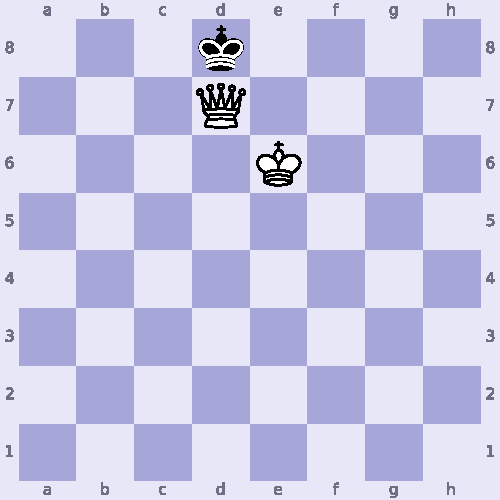
\includegraphics[height=3.1cm]{assets/board-witness}\\[4pt]
      {\small 종국 포지션 --- 킹·퀸 대 킹}\\[2pt]
      {\scriptsize\color{lcaccent}
       마지막 수는 폰 이동도 포획도 아닌 \emph{조용한} 체크메이트,\\
       그 순간 클록이 정확히 $150$}
    \end{column}
  \end{columns}
  \note{규모를 짚고 가겠습니다. 보통의 토너먼트 대국이 40수, 즉 80플라이
  안팎입니다. 왼쪽 격자에서 붉은 칸 하나가 그것이고, 최장 게임은 그것을 221판
  이어붙인 길이입니다.

  오른쪽이 그 게임이 실제로 끝나는 자리입니다. 킹과 퀸 대 킹. 마지막 수는 폰
  이동도 포획도 아닌 조용한 체크메이트인데, 그 순간 클록이 정확히 150입니다.
  9.6.2의 우선 조항이 없었다면 무승부로 끝났을 자리입니다.}
\end{frame}

% =========================================================== II. 계수
\lcpart{II}{계수}{$K \le 118$ --- 세는 것만으로}

\begin{frame}{정의}
  \centering
  \lcmap{2}
  \par\vspace{0.4cm}
  \begin{columns}[t]
    \begin{column}{0.485\textwidth}
      \begin{lcstate}{정의 2.1}{critical move}
        {\small 폰 이동 또는 포획. (앙파상은 둘 다, 승격은 폰 이동,
        캐슬링은 어느 쪽도 아니다.) 그 밖의 수를 \emph{quiet}이라 한다.}
      \end{lcstate}
      \begin{lcstate}{정의 2.2}{세그먼트 · endpoint}
        {\small critical move의 플라이를 $t_1<\dots<t_m$이라 하자.
        마지막 critical move 뒤에 quiet 플라이가 남으면 $T=1$, 아니면
        $T=0$. Endpoint는 $e_i=t_i$와 (필요시) $e_{m+1}=L$이며
        $K=m+T$.}
      \end{lcstate}
    \end{column}
    \begin{column}{0.485\textwidth}
      \begin{lcstate}{정의 2.3}{전환 수 $S$}
        {\small $e_i$의 \emph{색}은 그 플라이를 둔 쪽의 색이다.
        가상의 endpoint $e_0=0$은 관례상 흑.
        \[
          S=\#\{\,i\le K:\operatorname{col}(e_i)\ne
              \operatorname{col}(e_{i-1})\,\}.
        \]}
      \end{lcstate}
      \vspace{0.1cm}
      {\small critical move는 클록을 리셋하는 수와 정확히 일치하며,
      \emph{되돌릴 수 없다} --- 폰은 후퇴하지 못하고 잡힌 기물은 돌아오지
      않는다.}
    \end{column}
  \end{columns}
  \note{정의 셋을 깔겠습니다. 번호는 본문 그대로입니다.

  정의 2.1. critical move는 폰 이동 또는 포획입니다. 앙파상은 둘 다이고,
  승격은 폰 이동이며, 캐슬링은 어느 쪽도 아닙니다. 이것이 클록을 리셋하는
  수와 정확히 일치하고, 되돌릴 수 없다는 성질이 뒤에서 결정적입니다.

  정의 2.2. critical move들이 게임을 조각내고, 그 조각을 세그먼트라 합니다.
  마지막 critical move 뒤에 조용한 수가 남으면 종결 세그먼트가 하나 더
  붙습니다. 그것이 $T$이고, 세그먼트 개수가 $K$입니다.

  정의 2.3. 각 세그먼트의 마지막 플라이가 endpoint이고, 그 색은 그 수를 둔
  쪽의 색입니다. $S$는 그 색이 바뀌는 횟수인데, 게임 시작 지점에 가상의 흑
  endpoint가 있다고 치고 셉니다. 이 관례가 없으면 첫 세그먼트를 셀 수 없습니다.}
\end{frame}

\begin{frame}{보조정리 2.4 --- 세그먼트 분해}
  \centering
  \vspace{0.35cm}
  \begin{lcstate}{보조정리 2.4}{세그먼트 분해}
    \centering
    $L \;=\; 150K - S - \displaystyle\sum_{i=1}^{K}\delta_i,
     \qquad \delta_i \ge 0$\par\medskip
    {\small $\delta_i$는 세그먼트 $i$가 목표 길이(양 끝 같은 색이면 $150$,
    다르면 $149$)에 못 미친 양. 특히 $L \le 150K - S$.}
  \end{lcstate}
  \vspace{0.2cm}
  \begin{lcproof}
    \begin{lcsteps}
      \item 세그먼트 $i$의 플라이 중 마지막을 제외한 전부는 quiet이다.
        길이가 $151$ 이상이면 앞의 $150$개가 모두 quiet이 되어 그 지점에서
        게임이 이미 끝난다 (Art.~9.6.2) --- 모순. 따라서 길이 $\le 150$.
      \item 플라이는 색이 번갈아 오므로 세그먼트 길이가 짝수인 것과 양 끝
        endpoint의 색이 같은 것은 동치. 색이 다르면 길이가 홀수이고
        $\le150$이므로 $\le149$.
      \item 세그먼트 길이를 모두 더하면 $e_K-e_0=L$로 망원합된다. \qedhere
    \end{lcsteps}
  \end{lcproof}
  \note{보조정리 2.4가 발표 전체의 회계 장부입니다.

  증명은 세 단계입니다.

  1단계. 세그먼트 하나는 150플라이를 넘을 수 없습니다. 넘는다면 앞의 150개가
  전부 조용한 수가 되고, 9.6.2에 의해 거기서 이미 게임이 끝났어야 하니까요.

  2단계가 $S$가 등장하는 이유인데, 다음 장에서 그림으로 보겠습니다.

  3단계는 망원합입니다. 세그먼트 길이를 다 더하면 전체 길이가 됩니다.

  결론은 $L \le 150K - S$. 이제 $K$와 $S$를 각각 잡으면 됩니다.}
\end{frame}

\begin{frame}{보조정리 2.4의 2단계 --- 패리티}
  \centering
  \vspace{0.55cm}
  \figparity
  \par\vspace{0.6cm}
  {\small 플라이는 색이 번갈아 온다 $\;\Longrightarrow\;$
   세그먼트 길이의 홀짝 $=$ 양 끝 endpoint 색의 일치 여부}
  \note{순전히 패리티입니다.

  위 그림은 앞서 본 클록 그래프와 같은 어법입니다. 한 세그먼트 동안 클록이
  올라가고, 마지막 critical move에서 0으로 떨어집니다. 축 아래 띠가 각
  플라이의 색입니다.

  위 줄. 양 끝 endpoint의 색이 같으면 그 사이 플라이 수가 짝수여야 합니다.
  150은 짝수이므로 꽉 채울 수 있습니다.

  아래 줄. 양 끝 색이 다르면 길이가 홀수여야 하고, 150 이하 홀수의 최댓값은
  149입니다. 그래서 색이 바뀔 때마다 정확히 한 플라이를 잃습니다.

  이것이 분해식에 $S$가 그대로 들어가는 이유의 전부입니다.}
\end{frame}

\begin{frame}{critical move의 계수}
  \centering
  \vspace{0.05cm}
  {\large $K \;=\; (P - O) \;+\; (C + T)$}
  \par\vspace{0.3cm}
  \figaccount
  \par\vspace{0.35cm}
  {\small $P$ 폰 이동 \quad $C$ 포획 \quad
   $O$ 둘 다인 수 (대각선 폰 포획, 앙파상 포함) \quad
   $T$ 종결 세그먼트 $\in\{0,1\}$}
  \note{critical move의 개수를 포함배제로 셉니다.

  critical move는 폰 이동이거나 포획이므로, 그 총수는 폰 이동 수 더하기 포획
  수 빼기 둘 다인 수입니다. 둘 다인 수가 대각선 폰 포획이고, 이것을 겹침
  $O$라 합니다. 거기에 종결 세그먼트가 있으면 하나 더 붙습니다.

  묶는 방식이 중요합니다. $P-O$와 $C+T$로 묶으면 두 덩어리를 완전히 따로
  잡을 수 있습니다.

  그리고 이것을 \emph{모든} 게임에 대해 보여야 합니다. 알려진 구성을 보고
  ``겹침이 8개니까 96 빼기 8''이라고 하면 순환논법입니다. 그 구성이 최적인지가
  지금 증명하려는 것이니까요. 다음 네 장이 그 작업입니다.}
\end{frame}

\begin{frame}{보조정리 3.1 --- 폰 하나의 예산}
  \centering
  \vspace{0.2cm}
  \begin{columns}[c]
    \begin{column}{0.44\textwidth}\centering
      \figpawnfull
    \end{column}
    \begin{column}{0.53\textwidth}
      \begin{lcstate}{보조정리 3.1}{폰 기본}
        {\small 각 폰은 최대 $6$번의 폰 이동을 하므로 $P \le 96$.
        정확히 $6$번 움직인 폰은 매번 딱 한 랭크씩 전진하고 \emph{승격한다}.}
      \end{lcstate}
      \begin{lcproof}
        {\small 모든 폰 이동은 최소 한 랭크를 전진시키고, 홈 랭크와 승격
        랭크 사이에는 여섯 랭크가 있다. 여섯 번 움직였다면 매 이동이 정확히
        한 랭크였고 승격 랭크에 도달한 것이며, 승격은 의무다. \qed}
      \end{lcproof}
    \end{column}
  \end{columns}
  \par\vspace{0.25cm}
  {\small\color{lcaccent}
   따름: $P = 96$은 ``$16$개 폰 전부가 두 칸 전진 없이 여섯 번 걸어 전부
   승격했다''와 동치이다.}
  \note{가장 쉬운 것부터.

  폰 하나는 홈 랭크와 승격 랭크 사이에 여섯 랭크가 있고 모든 폰 이동은 최소
  한 랭크를 전진시킵니다. 그러니 폰당 최대 6수, 16개니까 $P \le 96$.

  딸려오는 따름이 훨씬 중요합니다. 어떤 폰이 정확히 여섯 번 움직였다면 그
  여섯 번이 전부 한 랭크씩이었다는 뜻이고, 결국 승격 랭크에 도착했다는
  뜻입니다. 승격은 의무니까 승격까지 했습니다.

  즉 $P = 96$은 ``16개 폰 전부가 두 칸 전진 한 번 없이 여섯 번 걸어서 전부
  승격했다''와 같은 말입니다. 판 위에 폰이 하나도 남지 않는다는 뜻이기도
  합니다. 뒤에서 계속 씁니다.}
\end{frame}

\begin{frame}{보조정리 3.3 --- unresolved origin pair}
  \centering
  \vspace{0.15cm}
  \begin{columns}[c]
    \begin{column}{0.24\textwidth}\centering
      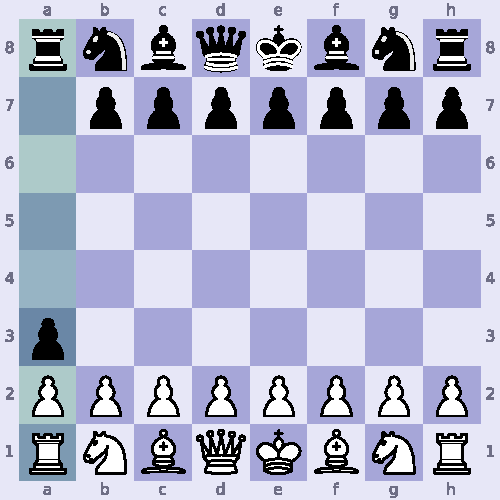
\includegraphics[width=\linewidth]{assets/board-cap10a}\\[2pt]
      \lccap{4\ldots a3 이후: 흑 $4$수}
    \end{column}
    \begin{column}{0.24\textwidth}\centering
      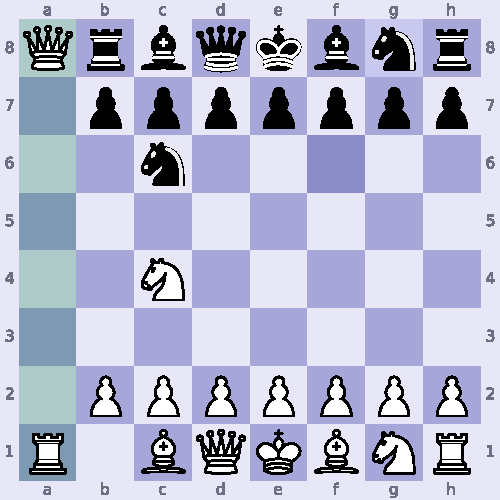
\includegraphics[width=\linewidth]{assets/board-cap10b}\\[2pt]
      \lccap{a8=Q 이후: 백 $6$수}
    \end{column}
    \begin{column}{0.48\textwidth}
      \begin{lcstate}{정의 3.2 · 보조정리 3.3}{}
        {\small 파일 $i$에서 시작하는 두 폰이 그 파일의 \emph{origin pair};
        둘 중 하나라도 대각선 폰 이동을 하면 그 파일은 \emph{resolved},
        아니면 \emph{unresolved}. resolved 파일 수를 $f$라 한다.\par\medskip
        \textbf{unresolved pair의 폰 이동 합은 최대 $10$이고, $10$은
        달성된다.}}
      \end{lcstate}
      \begin{lcproof}
        {\small 둘 다 판 위에 있는 동안 백 폰은 $2+a$, 흑 폰은 $7-b$ 랭크에
        있고 서로 지나칠 수 없으므로 $2+a<7-b$, 즉 $a+b\le4$. 한쪽이 (제3의
        기물에) 잡히면 그 기여는 $d\le4$로 고정되고 생존자는 보조정리 3.1로
        최대 $6$: 합 $d+6\le10$. \qed}
      \end{lcproof}
    \end{column}
  \end{columns}
  \par\vspace{0.2cm}
  {\small\color{lcaccent}\textbf{주의 3.4.}
   ``합계 $4$''는 \emph{둘 다 판 위에 있는 동안}만 참이다.
   전 게임 상한으로 쓰면 합법인 게임을 배제하게 된다.}
  \note{한 파일에서 마주 보고 시작하는 백 폰과 흑 폰을 그 파일의 origin
  pair라 합니다. 둘 다 한 번도 대각선으로 움직이지 않으면 그 파일을
  unresolved라 하고, resolved 파일의 개수를 $f$라 둡니다.

  둘 다 판 위에 있는 동안은 서로 지나칠 수 없습니다. 서로를 잡으려면
  대각선이어야 하는데 정의상 없고, 앞지르지도 못합니다---막힌 칸으로 밀 수
  없고 두 칸 점프로 넘을 수도 없으니까요. 그래서 합쳐서 4수까지입니다.

  그런데 한쪽이 제3의 기물에게 잡히면 남은 쪽이 자유로워집니다. 왼쪽 판에서
  흑 a폰이 네 칸 내려와 나이트에게 잡히고, 오른쪽에서 백 a폰이 파일 전체를
  걸어 승격합니다. 4가 아니라 10입니다.

  주의 3.4를 본문에 따로 실은 이유가 있습니다. 제 초기 모델이 여기서
  틀렸습니다. 4를 전 게임 상한으로 쓰면 합법인 게임을 배제해버립니다.}
\end{frame}

\begin{frame}{명제 3.6 --- $P - O \le 88$}
  \centering
  \vspace{0.15cm}
  \begin{columns}[c]
    \begin{column}{0.46\textwidth}\centering
      \figpminuso
    \end{column}
    \begin{column}{0.50\textwidth}
      \begin{lcstate}{보조정리 3.5}{겹침의 하한}
        {\small $O \ge f$. \ (resolved 파일마다 그 파일 출신 폰의 대각선
        이동을 하나씩 고르면, 이동자가 서로 달라 겹침이 서로 다르다.)}
      \end{lcstate}
      \begin{lcstate}{명제 3.6}{}
        {\small $P \le \min(96,\;80+2f)$이므로
        \[
          P - O \;\le\; \min(96,\,80+2f) - f \;\le\; \mathbf{88},
        \]
        등호는 오직 $f=8,\;P=96,\;O=8$에서만 성립한다.}
      \end{lcstate}
    \end{column}
  \end{columns}
  \par\vspace{0.25cm}
  {\small\color{lcaccent}
   $f$에 대해 최댓값을 취하는 이 단계가 명제를 ``겹침이 8개인 게임''이 아니라
   \emph{모든 게임}에 대한 진술로 만든다.}
  \note{천장이 둘입니다.

  하나. unresolved 파일마다 10, resolved 파일마다 12이므로 $10(8-f)+12f =
  80+2f$. 그림의 실선입니다.

  둘. 폰당 6이라는 절대 한도 96. 점선입니다.

  그런데 resolved 파일마다 대각선 폰 이동이 최소 하나 있고 그것은 포획이므로
  겹침입니다. 서로 다른 파일의 것은 서로 다른 수이므로 $O \ge f$. 파일을 하나
  풀 때마다 겹침을 하나씩 지불해야 한다는 뜻입니다.

  빼면 굵은 선이고, $f$가 8일 때 88에서 최댓값을 가지며 다른 곳에서는 더
  작습니다.

  $f$에 대해 최댓값을 취하는 이 단계가 결정적입니다. 이것이 있어야 특정 게임이
  아니라 모든 게임에 대한 명제가 됩니다.}
\end{frame}

\begin{frame}{보조정리 3.7 --- $C + T \le 30$}
  \centering
  \vspace{0.25cm}
  \begin{columns}[c]
    \begin{column}{0.28\textwidth}\centering
      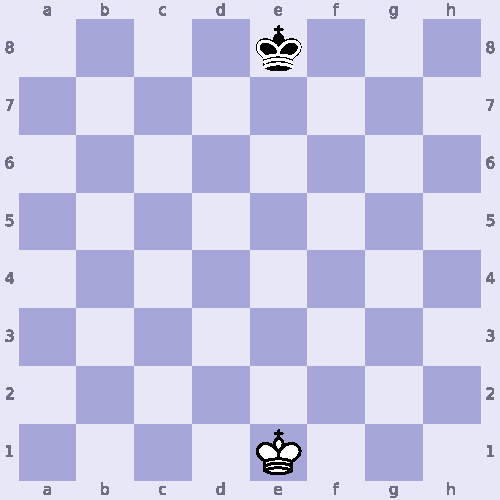
\includegraphics[width=0.88\linewidth]{assets/board-barekings}\\[3pt]
      \lccap{킹 대 킹: dead position}
    \end{column}
    \begin{column}{0.66\textwidth}
      \begin{lcstate}{보조정리 3.7}{}
        {\small $C + T \le 30$.}
      \end{lcstate}
      \begin{lcproof}
        \begin{lcsteps}
          \item 킹이 아닌 기물은 $30$개뿐이므로 $C \le 30$.
          \item $C \le 29$이면 $T \le 1$에서 곧바로 $C+T \le 30$.
          \item $C = 30$이면 $30$번째 포획이 킹 둘만 남긴다. 킹 대 킹은
            dead position이므로 게임은 \emph{그 수에서} 끝나고, 뒤따르는
            quiet 플라이가 없어 $T = 0$. \qedhere
        \end{lcsteps}
      \end{lcproof}
    \end{column}
  \end{columns}
  \par\vspace{0.3cm}
  {\small
   $\underbrace{96+30-8+0}_{\text{30개 다 잡음}} \;=\;
    \underbrace{96+29-8+1}_{\text{29개, 종결 세그먼트}} \;=\; 118$
   \qquad 어느 쪽으로 가도 이득이 없다.}
  \note{포획은 최대 30입니다. 킹은 잡히지 않으니까요.

  그런데 30을 다 채우면 킹 둘만 남습니다. 킹 대 킹은 dead position입니다.
  어떤 합법 수순으로도 체크메이트가 불가능하니까요. 그러면 그 포지션이 생기는
  순간 게임이 끝나고, 뒤에 조용한 수가 따라올 수 없어 $T=0$입니다.

  그래서 $C+T \le 30$. 아래 식이 보여주듯 30번 다 잡고 종결 세그먼트를
  포기하거나 29번만 잡고 종결 세그먼트를 얻거나, 둘 다 118입니다.

  덧붙이면 이 증명 전체에서 dead position 논증이 등장하는 곳은 여기 한 번뿐이고,
  킹 대 킹은 deadness에 이견이 있을 수 없는 유일한 경우입니다.}
\end{frame}

\begin{frame}{정리 3.8 --- $K \le 118$}
  \centering
  \vspace{0.15cm}
  \begin{lcthm}{정리 3.8}{}
    \centering
    {\small 모든 게임은 $K = (P-O)+(C+T) \le 88 + 30 = \mathbf{118}$을
    만족한다. 나아가 $K = 118$인 게임은
    $f = 8$, \ $P = 96$, \ $O = 8$, \ $C + T = 30$이며, 따라서
    \emph{16개 폰 전부가 여섯 번 움직여 승격하고} $C \ge 29$이다.}
  \end{lcthm}
  \vspace{0.15cm}
  \begin{columns}[c]
    \begin{column}{0.30\textwidth}\centering
      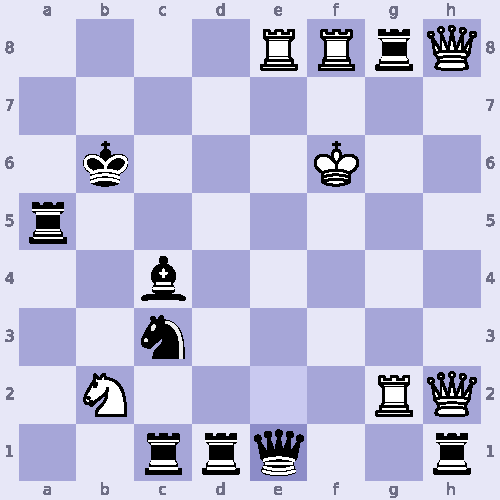
\includegraphics[width=0.86\linewidth]{assets/board-nopawns}\\[2pt]
      \lccap{실제 기보, 마지막 폰 이동 직후 --- 폰이 없다}
    \end{column}
    \begin{column}{0.64\textwidth}
      \begin{lcstate}{주의 3.9}{Murphy의 천장}
        {\small $K=118 \Rightarrow P=96 \Rightarrow$ 양쪽 다 폰을 움직임
        $\Rightarrow$ 양색 endpoint 존재 $\Rightarrow S \ge 1$, 즉
        \[ L \;\le\; 150\cdot118 - 1 \;=\; 17{,}699. \]}
      \end{lcstate}
      {\small\color{lcaccent}남은 두 플라이가 어려운 부분이며,
       III부 전체가 그것이다.}
    \end{column}
  \end{columns}
  \note{합치면 118입니다.

  등호일 때가 훨씬 유익합니다. $88+30$에서 등호가 되려면 양쪽 다 등호여야
  하고, 명제 3.6의 등호 조건이 $f=8$, $P=96$, $O=8$을 못 박습니다.

  $P=96$은 앞서 보았듯 16개 폰 전부가 승격했다는 뜻입니다. 왼쪽이 실제 기보에서
  마지막 폰 이동 직후의 포지션인데, 정말로 폰이 없고 승격한 룩과 퀸이 널려
  있습니다. 그리고 $T \le 1$에서 $C \ge 29$.

  주의 3.9. 여기서 공짜로 하나 나옵니다. $P=96$이면 양쪽 다 폰을 움직이고,
  폰 이동은 그 폰 주인의 critical move이므로 양쪽 색의 endpoint가 다
  존재합니다. 가상의 $e_0$가 흑인데 어딘가 백 endpoint가 있으니 색이 최소 한
  번은 바뀝니다. 그래서 17{,}699---Murphy의 천장이 이제 모든 게임에 대한
  정리가 되었습니다.

  기억하실 것은 두 개입니다. $P=96$과 $C\ge29$. III부의 모든 논증이 이 둘
  위에서 돌아갑니다.}
\end{frame}

% =========================================================== III. 전환
\lcpart{III}{전환}{$K = 118$이면 $S \ge 3$}

\begin{frame}{블록과 패턴}
  \centering
  \lcmap{3}
  \par\vspace{0.4cm}
  \begin{columns}[c]
    \begin{column}{0.53\textwidth}\centering
      \begin{tikzpicture}[x=1mm,y=1mm,font=\scriptsize]
        \foreach \c [count=\i from 0] in {B,B,B,W,W,B,B,W,W,W,W,B} {
          \path[seg\c] ({\i*6.2},0) rectangle ++(5.9,4.5);}
        \draw[lcarrow] (37,-3) -- (37,-9);
        \foreach \c/\s/\e in {B/0/2, W/3/4, B/5/6, W/7/10, B/11/11} {
          \path[seg\c,rounded corners=1pt]
            ({\s*6.2},-19) rectangle ({\e*6.2+5.9},-14);}
        \node[anchor=west,font=\tiny,text=lcgrey] at (78,2.2)
          {critical move 열};
        \node[anchor=west,font=\tiny,text=lcgrey] at (78,-16.5)
          {패턴 $\B\W\B\W\B$};
      \end{tikzpicture}
    \end{column}
    \begin{column}{0.44\textwidth}
      \begin{lcstate}{정의}{블록 · 패턴}
        {\small 각 critical move를 그 수를 둔 쪽 색으로 칠하고, 같은 색의
        최대 연속 구간을 \emph{블록}이라 한다. 블록 색의 나열이
        \emph{패턴}이다. Endpoint 열에 대해 같게 하면 \emph{endpoint 패턴}.}
      \end{lcstate}
      \begin{lcstate}{관찰}{}
        {\small endpoint 블록이 $n$개면
        $S = n-1$ (흑으로 시작) 또는 $S = n$ (백으로 시작).\par\medskip
        \textcolor{lcaccent}{따라서 $S \le 2$를 배제하려면 3블록 이하
        패턴을 전부 죽이면 된다.}}
      \end{lcstate}
    \end{column}
  \end{columns}
  \note{용어를 하나 더 도입합니다.

  critical move 하나하나를 그 수를 둔 쪽 색으로 칠합니다. 폰 이동은 그 폰
  주인의 색, 포획은 잡은 쪽의 색입니다.

  그러면 색깔 열이 하나 나오는데, 같은 색이 이어지는 최대 구간을 블록이라
  하고 블록 색만 나열한 것을 패턴이라 합니다. 왼쪽 위가 열, 아래가 패턴입니다.

  endpoint에 대해서도 같게 하면 endpoint 패턴입니다. 블록이 $n$개면 전환 횟수
  $S$는 $n-1$ 아니면 $n$입니다. 흑으로 시작하면 $n-1$, 백으로 시작하면 가상의
  흑 $e_0$와 한 번 더 부딪히므로 $n$입니다.

  따라서 $S \le 2$를 배제하는 일은 블록 3개 이하인 패턴을 전부 배제하는 일과
  같습니다.}
\end{frame}

\begin{frame}{3블록 이하 패턴은 여섯 가지뿐}
  \centering
  \vspace{0.95cm}
  \figpatterns
  \par\vspace{1.05cm}
  {\small 여섯을 모두 배제하면 모든 패턴이 최소 네 블록,
   따라서 $S \ge 3$이다.}
  \note{비어 있지 않은, 색이 번갈아 나오는, 블록 세 개 이하인 패턴은 정확히
  여섯 가지입니다. B, W, BW, WB, BWB, WBW. 이것이 전부입니다.

  이 여섯을 $K=118$에서 전부 불가능하다고 보이면 모든 패턴이 최소 네 블록이고,
  따라서 $S \ge 3$입니다.

  앞의 넷은 세는 것만으로 죽습니다. 뒤의 두 개, 3블록짜리가 어렵고 여기에
  보조정리가 하나 필요합니다.

  결과를 먼저 말씀드리면 살아남는 것은 BWBW 하나이고, 그것이 정확히 실제
  기보의 패턴입니다.}
\end{frame}

\begin{frame}{명제 4.1 · 4.2 --- 1블록과 2블록}
  \centering
  \vspace{0.1cm}
  \begin{columns}[t]
    \begin{column}{0.485\textwidth}
      \begin{lcstate}{명제 4.1}{1블록}
        {\small $K=118$에서 $\B$, $\W$는 불가능하다.\par\smallskip
        \emph{증명.} 한 색만 critical move를 두면 그쪽 폰 여덟 개만
        움직이므로 $P \le 48 < 96$. \qed}
      \end{lcstate}
      \begin{lcstate}{명제 4.2}{2블록}
        {\small $\B\W$, $\W\B$도 불가능하다.\par\smallskip
        \emph{증명.} 패턴을 $(X,Y)$라 하면 $Y$는 $X$의 포획 가능 기물
        $15$개만 잡을 수 있어 $C_Y \le 15$, 따라서
        $C_X \ge 29-15 = 14$. 그 $\ge14$개는 $Y$의 첫 critical move
        \emph{이전}에 잡히므로 폰 이동을 한 번도 하지 못한다. 그중 폰 출신이
        아닌 것은 최대 $7$개이므로 폰 $\ge7$개가 자기 $6$수를 전부 잃는다.
        \qed}
      \end{lcstate}
    \end{column}
    \begin{column}{0.485\textwidth}\centering
      \vspace{0.2cm}
      \figtwoblocks
      \par\vspace{0.45cm}
      \scalebox{0.66}{\figpawngrid{6}{7}{54}}
    \end{column}
  \end{columns}
  \note{명제 4.1은 한 줄입니다. 한 색만 critical move를 두면 그쪽 폰 여덟
  개만 움직입니다. $P \le 48$인데 96이 필요하니 끝입니다.

  명제 4.2가 조금 더 흥미롭습니다. 패턴을 $(X, Y)$라 하면 $X$의 모든 critical
  move가 $Y$의 모든 critical move보다 앞섭니다.

  $Y$는 $X$의 기물만 잡을 수 있고 그것은 15개뿐이므로 $C_Y \le 15$. 그런데
  $C \ge 29$였으니 $C_X \ge 14$. 먼저 두는 쪽이 최소 14번 잡는데, 전부 $Y$가
  critical move를 하나라도 두기 전입니다.

  그러면 그 14개는 판에서 사라진 뒤에야 $Y$의 첫 critical move가 오므로 폰
  이동을 한 번도 하지 못한 것입니다. 그중 폰 출신이 아닌 것은 최대 7개---퀸,
  룩 둘, 비숍 둘, 나이트 둘. 그러니 최소 7개는 폰 출신이고 각각 자기 6수를
  통째로 잃습니다.

  오른쪽 아래 격자가 그것입니다. 42칸이 날아가 $P \le 54$. 96에 한참
  못 미칩니다.}
\end{frame}

\begin{frame}{보조정리 4.3 --- home-rank 보조정리}
  \centering
  \vspace{0.15cm}
  \begin{columns}[c]
    \begin{column}{0.33\textwidth}\centering
      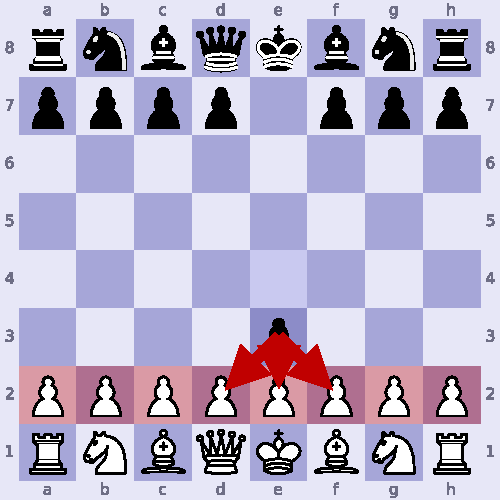
\includegraphics[width=0.92\linewidth]{assets/board-homerank}\\[2pt]
      \lccap{1.\,Nf3 e6\ 2.\,Ng1 e5\ 3.\,Nf3 e4\ 4.\,Ng1 e3}
    \end{column}
    \begin{column}{0.61\textwidth}
      \begin{lcstate}{보조정리 4.3}{home-rank}
        {\small 공격자 $A$와 수비자 $D$를 고정하고, 초기 포지션에서
        다음을 만족하며 도달 가능한 포지션을 생각하자.
        \begin{itemize}\setlength{\itemsep}{1pt}
          \item[(R1)] $D$의 모든 수는 quiet이고,
          \item[(R2)] $A$의 어떤 수도 $D$의 폰을 잡지 않는다.
        \end{itemize}
        그러면 $D$의 폰 홈 랭크는 \emph{한 칸도 변하지 않고}, $A$의 폰은
        그 랭크에 설 수 없으며, \textcolor{lcaccent}{$A$의 어떤 폰도 폰
        이동을 네 번 넘게 하지 못한다.}}
      \end{lcstate}
    \end{column}
  \end{columns}
  \par\vspace{0.25cm}
  {\small 판의 흑 폰은 e3에서 멈춘다: e2를 치울 수 있는 것은 백뿐이고(R1 위반),
   뚫을 수 있는 것은 d2·f2 포획뿐이다(R2 위반).}
  \note{여기가 논문의 심장입니다.

  상황은 이렇습니다. 공격자 $A$와 수비자 $D$가 있는데, $D$는 조용한 수만 두고
  $A$는 $D$의 폰을 잡지 않는다.

  판을 보시면 흑 폰이 e3까지 네 칸 내려와 멈춰 있습니다. 갈 데가 없습니다.

  e2에는 백 폰이 있습니다. 그것을 치울 수 있는 것은 백뿐인데 폰을 움직이는 것은
  조용한 수가 아니므로 (R1) 위반입니다. 밀어서는 못 갑니다---막혀 있으니까요.
  대각선으로 d2나 f2를 잡아야 하는데 그것이 정확히 (R2)가 금지하는 것입니다.

  그래서 홈 랭크가 통째로 벽이 됩니다. 한 칸도 변하지 않습니다.

  증명의 나머지와 왜 하필 네 수인지는 다음 장입니다.}
\end{frame}

\begin{frame}{보조정리 4.3의 증명}
  \centering
  \vspace{0.15cm}
  \begin{columns}[c]
    \begin{column}{0.26\textwidth}\centering
      \fighomeranks
    \end{column}
    \begin{column}{0.68\textwidth}
      \begin{lcproof}
        \begin{lcsteps}
          \item \emph{$D$의 홈 랭크는 불변.} 수에 대한 귀납. 어떤 수도 그
            칸에서 \emph{시작}할 수 없다---$D$ 폰이 있고 그것을 움직이는 것은
            (R1) 위반. \emph{끝날} 수도 없다---점유된 칸이므로 포획이어야
            하는데 $D$의 포획은 (R1), $A$의 폰 포획은 (R2) 위반.
            캐슬링은 백 랭크만, 앙파상은 랭크 $4$·$5$만 건드린다.
          \item \emph{$A$의 폰은 $D$의 홈 랭크에 설 수 없다.} 거기서
            끝나는 수가 (1)에서 배제되었다.
          \item \emph{따라서 최대 네 수.} 그 너머 랭크는 $D$의 홈 랭크에서
            한 칸 밀거나 자기 홈 랭크가 아닌 곳에서 두 칸 뛰어야 도달하는데
            둘 다 불가능. 사정거리는 네 랭크이고 폰 이동 하나가 최소 한
            랭크를 쓴다. \qedhere
        \end{lcsteps}
      \end{lcproof}
    \end{column}
  \end{columns}
  \par\vspace{0.15cm}
  {\scriptsize\color{lcgrey}
   귀납에 쓰이는 것은 합법 수의 기초 사실 [H0]--[H6]뿐이다:
   어떤 수가 어떤 칸의 점유를 바꿀 수 있는가, 폰은 어떻게 전진하는가.}
  \note{벽이 변하지 않는다는 것을 알면 나머지는 셈입니다.

  1단계가 벽입니다. 어떤 수도 그 칸에서 시작할 수 없고, 끝날 수도 없습니다.
  캐슬링과 앙파상은 따로 확인합니다.

  2단계. $A$의 폰은 $D$의 홈 랭크에 설 수 없습니다. 거기서 끝나는 수가 방금
  배제되었으니까요.

  3단계. 그 너머, 즉 승격 랭크 쪽도 못 갑니다. 거기 가려면 $D$의 홈 랭크에서
  한 칸 밀고 나가거나 자기 홈 랭크가 아닌 곳에서 두 칸을 뛰어야 하는데, 전자는
  홈 랭크에 설 수 없으니 불가능하고 후자는 규칙상 불가능합니다.

  그러니 $A$의 폰이 쓸 수 있는 것은 자기 홈 랭크와 $D$의 홈 랭크 사이 네
  랭크뿐이고, 폰 이동 하나가 최소 한 랭크를 쓰므로 최대 네 수입니다. 그리고
  네 수는 실제로 달성됩니다.}
\end{frame}

\begin{frame}{명제 4.4 --- 3블록 $(X, Y, X)$}
  \centering
  \vspace{0.1cm}
  \begin{columns}[t]
    \begin{column}{0.50\textwidth}
      \begin{lcstate}{명제 4.4}{}
        {\small $K=118$에서 $\B\W\B$, $\W\B\W$는 불가능하다.}
      \end{lcstate}
      \begin{lcproof}
        \begin{lcsteps}
          \item 앞과 같이 $C_Y \ge 14$이고 이 포획은 전부 가운데 블록에
            있다. 희생자 중 $\ge7$개는 폰으로 시작한 $X$-기물이다.
          \item 그런 기물 $p$의 여섯 폰 이동은 전부 $Y$의 첫 critical move
            $\tau$ \emph{이전}이다. $\tau$ 이후의 $X$-critical move는 마지막
            블록에 속하고, 그것은 $p$가 잡힌 뒤이기 때문이다.
          \item 첫 구간은 보조정리 4.3의 상황이다: (R1)은 $\tau$의 정의,
            (R2)는 $P=96$에서 나온다. 따라서 $X$ 폰당 최대 \emph{네} 수.
            \qedhere
        \end{lcsteps}
      \end{lcproof}
    \end{column}
    \begin{column}{0.47\textwidth}\centering
      \vspace{0.15cm}
      \figthreeblocks
      \par\vspace{0.2cm}
      \scalebox{0.58}{\figpawngrid{2}{7}{82}}
    \end{column}
  \end{columns}
  \note{이제 3블록을 배제합니다.

  1단계는 앞과 같습니다. $C_Y \ge 14$이고, $Y$의 critical move는 전부 가운데
  블록에 있으므로 그 포획들도 전부 거기 있습니다. 희생자 중 최소 7개는 $X$의
  폰 출신 기물입니다.

  2단계. 그런 기물 하나를 $p$라 합시다. $p$는 여섯 번 폰 이동을 해야 하는데
  전부 자기가 잡히기 전에 해야 합니다. 그런데 $Y$의 첫 critical move 시점
  $\tau$ 이후의 $X$ critical move는 전부 마지막 블록에 속하고, 그것은 $p$가
  잡힌 뒤입니다. 판에 없는 기물은 움직이지 못합니다. 따라서 여섯 수가 전부
  첫 구간에 있어야 합니다.

  3단계. 첫 구간이 정확히 보조정리 4.3의 상황입니다. (R1)은 $\tau$의 정의에서
  바로 나오고, (R2)는 $P=96$에서 나옵니다---$X$가 $Y$의 폰을 잡았다면 그 폰은
  폰 이동을 한 번도 못 하니까요.

  그러면 $X$의 폰은 첫 구간에서 최대 네 수. 여섯이 필요한데 넷입니다. 7개 폰이
  각각 2씩 모자라 $P \le 82$입니다.}
\end{frame}

\begin{frame}{정리 4.5 --- $S \ge 3$}
  \centering
  \vspace{0.45cm}
  \begin{lcthm}{정리 4.5}{네 블록}
    \centering
    {\small $K = 118$인 모든 게임의 critical-move 패턴은 최소 네 블록이다.
    Endpoint 열은 critical-move 열에 원소를 최대 하나 덧붙인 것이므로 블록
    수가 줄지 않고, 따라서 endpoint 패턴도 최소 네 블록이며 $\;S \ge 3$.}
  \end{lcthm}
  \vspace{0.5cm}
  \begin{tikzpicture}[x=1mm,y=1mm,font=\scriptsize]
    \node[lcbox] (a) at (0,0) {$\B$, $\W$\\ 명제 4.1};
    \node[lcbox] (b) at (32,0) {$\B\W$, $\W\B$\\ 명제 4.2};
    \node[lcboxa] (c) at (66,0) {$\B\W\B$, $\W\B\W$\\ 명제 4.4};
    \node[lcboxk] (d) at (104,0) {$\ge4$ 블록\\ $S \ge 3$};
    \draw[lcarrow] (a) -- (d); \draw[lcarrow] (b) -- (d);
    \draw[lcarrow] (c) -- (d);
  \end{tikzpicture}
  \par\vspace{0.5cm}
  {\small\color{lcgrey}
   \textbf{주의 4.6.} $S \ge 3$은 \emph{오직} $K = 118$ 아래에서만 참이다.
   1.\,Nf3 Nf6 2.\,Ng1 Ng8을 네 번 반복하면 $K = 1$, $S = 0$인 16플라이
   게임이 된다.}
  \note{여섯을 모두 배제했으므로 블록이 최소 넷입니다.

  endpoint 열은 critical move 열 뒤에 종결 endpoint가 최대 하나 붙은
  것인데, 붙어도 블록 수가 줄지는 않습니다. 그러니 endpoint 패턴도 최소 네
  블록이고 $S \ge 3$입니다.

  주의 4.6을 강조하겠습니다. $S \ge 3$은 $K = 118$이라는 가정 아래에서만
  참입니다. 일반적으로는 명백히 거짓입니다. Nf3 Nf6 Ng1 Ng8을 네 번 반복하면
  16플라이 만에 초기 포지션 5회 반복으로 끝나는데, 폰 이동도 포획도 없으니
  $K=1$이고 $S=0$입니다.

  그래도 상관없습니다. $K \le 117$이면 세그먼트를 통째로 하나 잃는 것이라
  어떤 전환 횟수로도 만회되지 않습니다.}
\end{frame}

\begin{frame}{정리 5.1 --- 상한}
  \centering
  \vspace{0.4cm}
  \begin{lcthm}{정리 5.1}{상한}
    \centering 어떤 합법 체스 게임도 $17{,}697$ 플라이를 넘지 못한다.
  \end{lcthm}
  \vspace{0.3cm}
  \begin{lcproof}
    {\small
    \begin{tabular}{@{}ll@{}}
      $K \le 117$ & 보조정리 2.4와 $S \ge 0$에서 \
                    $L \;\le\; 150 \cdot 117 \;=\; 17{,}550 \;<\; 17{,}697$ \\[5pt]
      $K = 118$   & 정리 3.8이 허용하는 최댓값. 정리 4.5의 $S \ge 3$에서 \
                    $L \;\le\; 150 \cdot 118 - 3 \;=\; \mathbf{17{,}697}$ \\
    \end{tabular}\par\medskip
    \hfill\qed}
  \end{lcproof}
  \vspace{0.3cm}
  \begin{lcthm}{따름정리 5.3}{정확한 최댓값}
    \centering
    {\small 상한은 달성된다 (Labelle의 생성 기보, Murphy의 수제 기보).
    \textbf{체스 게임의 최대 길이는 정확히 $17{,}697$ 플라이,
    즉 $8{,}848$수와 백의 마지막 한 수이다.}}
  \end{lcthm}
  \note{증명은 두 줄입니다.

  $K \le 117$이면 세그먼트가 하나 없는 것이라 $150 \times 117 = 17{,}550$,
  17{,}697보다 작습니다.

  $K = 118$이면 방금 증명한 $S \ge 3$이 붙어 $150 \times 118 - 3 = 17{,}697$.

  두 경우를 분리해야 하는 것이 요점입니다. $S \ge 3$은 $K \le 117$에서 쓸 수
  없고, 쓸 필요도 없습니다---세그먼트 하나가 어떤 전환 횟수보다 무겁습니다.

  그리고 하한은 이미 있습니다. 공개된 기보 두 개가 정확히 이 길이입니다.
  그래서 최댓값이 정확히 17{,}697입니다. 부등식이 아니라 등식입니다.}
\end{frame}

\begin{frame}{따름정리 5.2 --- 최대 길이 게임의 구조}
  \centering
  \vspace{0.5cm}
  \begin{lcthm}{따름정리 5.2}{}
    \centering
    {\small 길이 $17{,}697$인 모든 게임은
    $K = 118$, \ $S = 3$, \ 모든 $\delta_i = 0$, \
    $f = 8$, \ $P = 96$, \ $O = 8$, \ $C + T = 30$을 만족하며,
    critical-move 패턴과 endpoint 패턴이 모두 $\B\W\B\W$이다.}
  \end{lcthm}
  \vspace{0.5cm}
  {\small
  16개 폰 전부가 여섯 번, 매번 한 랭크씩 전진해 승격 \quad$\cdot$\quad
  모든 세그먼트가 꽉 참 ($150$, 전환을 끼면 $149$)}
  \par\vspace{0.55cm}
  {\large \lcstrip{B,W,B,W}\ \ $\B\W\B\W$ \quad
   \textcolor{lcaccent}{흑이 첫 critical move를 두고,
   마지막 endpoint는 백의 수다.}}
  \note{등호 분석이 공짜로 따라옵니다.

  길이가 17{,}697이면 앞의 부등식이 전부 등식이어야 합니다. 그러면 $K=118$,
  $S$가 정확히 3, 모든 $\delta$가 0---세그먼트를 하나도 낭비하지 않았다는
  뜻입니다.

  거기서 등호 조건들이 전부 따라 나옵니다. 폰 16개 전원 승격, 겹침 정확히 8개.

  패턴도 결정됩니다. 블록이 정확히 넷이고, 백으로 시작할 수 없습니다---그러면
  가상의 흑 $e_0$와 한 번 더 부딪혀 $S \ge 4$가 되니까요. 그래서 BWBW입니다.

  즉 최대 길이 게임이 \emph{어떻게} 생겼는지까지 정해집니다. 흑이 먼저
  critical move를 두고 백이 마지막 수를 둡니다. 선택의 여지가 없습니다.}
\end{frame}

% =========================================================== IV. 탐색
\lcpart{IV}{탐색}{정리 이전의 시도}

\begin{frame}{탐색 1 --- 대량 생성}
  \centering
  \lcmap{4}
  \par\vspace{0.35cm}
  \figattackone
  \par\vspace{0.45cm}
  {\small 같은 $118$개 critical move, quiet filler만 새로 생성해 서로 다른
   $17{,}697$-플라이 게임을 대량 생산 $\rightarrow$
   전부에 대해 ``합법적인 한 수 더''를 검사}
  \note{시간 순서로는 이것이 먼저였습니다. 저는 17{,}697을 깨려 했습니다.

  첫 시도는 무식한 쪽입니다. 알려진 기보에서 출발해 critical move 118개는
  그대로 두고 사이를 채우는 조용한 수들만 새로 생성해, 서로 다른 17{,}697
  플라이 게임을 대량으로 만들었습니다. 그중 하나는 17{,}032 플라이가 원본과
  다릅니다.

  그리고 전부에 같은 질문을 던졌습니다. 여기에 합법적인 한 수를 더 붙일 수
  있는가.

  하나도 없었습니다. 매번 정확히 같은 벽에 부딪혔습니다.

  이것은 증명이 아닙니다. 다만 벽이 우연이 아니라는 신호였습니다.}
\end{frame}

\begin{frame}{탐색 2 --- 표적 탐색}
  \centering
  \vspace{0.55cm}
  \figattacktwo
  \par\vspace{1.05cm}
  {\small 가설: \emph{$118$개 세그먼트를 유지하면서 색 전환을 $2$회 이하로
   하는 합법 골격이 존재한다}}
  \par\vspace{0.45cm}
  {\color{lcaccent}\small 폰 이동·포획 예산에 대한 추상 CP-SAT 모델과
   후보를 실제 수순으로 실현할 플래너 --- 모든 인스턴스가 infeasible}
  \note{두 번째 시도는 표적을 정했습니다. 가설은 세그먼트 118개를 유지하면서
  색 전환을 두 번 이하로 하는 합법 골격이 존재한다는 것입니다.

  폰 이동과 포획 예산에 대한 추상 CP-SAT 모델을 짜고, 모델이 내놓는 후보를
  실제 수순으로 실현할 구체 플래너를 붙였습니다.

  모든 인스턴스가 infeasible이었습니다. 플래너는 할 일이 없었습니다.

  여기서 방향을 틀었습니다. 계속 찾지 못한다는 것은 없다는 뜻일 수 있으니까요.
  17{,}697을 깨야 할 목표가 아니라 증명해야 할 정리로 취급하기 시작했습니다.}
\end{frame}

\begin{frame}{증명의 구조}
  \centering
  \vspace{0.9cm}
  \figdag
  \par\vspace{1.1cm}
  {\small 여기까지 컴퓨터는 한 줄도 필요하지 않다.}
  \note{그래서 나온 증명이 이 모양입니다. 왼쪽이 폰과 포획에 대한 기초
  보조정리들, 가운데가 $K \le 118$, 오른쪽이 패턴 논증과 $S \ge 3$입니다.

  아래 상자가 $K \le 117$인 경우인데, 세그먼트가 부족해 17{,}550으로 끝납니다.

  강조하고 싶은 것은 여기까지 컴퓨터가 한 줄도 필요하지 않다는 점입니다. 전부
  손으로 검산 가능합니다. 다음 부에서 컴퓨터가 등장하는데, 증명을 대체하는
  것이 아니라 교차검증하는 것입니다.}
\end{frame}

% =========================================================== V. 검증
\lcpart{V}{검증}{계산은 증명을 대체하지 않는다}

\begin{frame}{계산의 역할}
  \centering
  \lcmap{5}
  \par\vspace{0.75cm}
  \figpipeline
  \par\vspace{0.95cm}
  {\small 위: 기보를 판정한다 \quad$\cdot$\quad
   아래: 손 논증을 두 가지 독립된 방법으로 교차검증한다
   (sound 방향만 --- infeasible만 결론에 쓰인다)}
  \note{컴퓨터가 하는 일이 두 가지입니다.

  위쪽. 독립 검증기가 Murphy의 기보를 초기 포지션부터 플라이 단위로 재생합니다.
  합법성, 조기 종료 여부, 매 플라이 이후의 포지션 분류를 전부 기록하고, 마지막
  수에서 정확히 끝나야만 통과시킵니다. 이 검증기는 저장소의 다른 코드를
  아무것도 import하지 않습니다. 판정하는 쪽과 만드는 쪽을 분리했습니다.

  아래쪽. 증명의 유한 경우분석을 기계로 전수 확인하고, 패턴 질문---블록 3개
  이하인 endpoint 패턴이 $K=118$을 허용하는가---을 두 가지 독립된 방법으로 다시
  답합니다. CP-SAT 모델 하나, solver 없이 자기 상수를 직접 선언하는 산술 검사기
  하나.

  둘 다 sound 방향으로만 씁니다. infeasible이면 그런 게임이 없다는 결론이
  나오지만, feasible이라고 게임이 존재한다는 결론은 내지 않습니다. 논문의 어떤
  주장도 feasible 판정에 기대지 않습니다.}
\end{frame}

\begin{frame}{검증기가 구현하는 두 규칙}
  \centering
  \vspace{0.6cm}
  \begin{columns}[t]
    \begin{column}{0.47\textwidth}
      \begin{lcstate}{체크메이트가 클록보다 우선}{}
        {\small 마지막 플라이는 그 세그먼트의 $150$번째 quiet 플라이이면서
        동시에 메이트다 (Art.~9.6.2의 우선 조항).\par\medskip
        클록을 먼저 판정하는 검증기는 같은 $17{,}697$ 플라이를 받아들이지만
        \alert{결과를 무승부로 적는다.}}
      \end{lcstate}
    \end{column}
    \begin{column}{0.47\textwidth}
      \begin{lcstate}{FEN 전체를 비교하지 말 것}{}
        {\small 반복 판정에서 클록과 수순 번호는 동일성과 무관하고,
        en passant은 \emph{합법}일 때만 센다 (Art.~9.2).\par\medskip
        \alert{양방향으로 다 틀린다} --- FEN은 너무 나누고, 배치$+$차례만
        보면 캐슬링 권리를 무시해 너무 합친다.}
      \end{lcstate}
    \end{column}
  \end{columns}
  \par\vspace{0.7cm}
  {\small 이 식별 아래에서 이 기보의 어떤 포지션도 \emph{세 번} 나오지
   않는다 --- 5회 반복은 근처에도 가지 않는다.}
  \note{이 둘은 엔지니어링 선택이 아니라 체스 규칙이고, 실제 기보가 둘 다
  건드립니다.

  첫째, 종료 판정 순서. 마지막 플라이는 그 세그먼트의 150번째 조용한 수이면서
  동시에 체크메이트입니다. 9.6.2의 우선 조항이 메이트를 살립니다. 클록을 먼저
  보는 검증기는 길이는 똑같이 17{,}697로 받아들이지만 결과를 무승부로 적습니다.
  길이는 맞고 결과가 틀립니다.

  둘째, 반복 판정의 포지션 동일성. FEN 문자열 전체를 비교하면 안 됩니다.
  하프무브 클록과 수순 번호는 동일성과 무관하고, en passant 타겟은 두 칸
  전진이 있으면 실제로 잡을 수 있든 없든 기록되니까요. 그러면 5회 반복이
  영원히 걸리지 않습니다. 반대로 배치와 차례만 보면 캐슬링 권리를 무시해 너무
  합쳐버립니다.

  참고로 Tom 7의 참조 구현에는 지금도 MOVE\_RULE이 50으로 박혀 있습니다. 75가
  맞다는 주석 바로 밑에요. 참조 구현은 신탁이 아니라는 것이 검증기를 독립적으로
  만든 이유입니다.}
\end{frame}

\begin{frame}{검증 결과와 재현}
  \centering
  \vspace{0.65cm}
  {\small
  \begin{tabular}{@{}ll@{}}
    \toprule
    기보 & 합법, $17{,}697$ 플라이, 체크메이트로 종료 \\
    조기 종료 & 없음 --- 어떤 포지션도 3회 미만, 스테일메이트 없음 \\
    프로필 & $K = 118$, $P = 96$, $C = 29$, $O = 8$, $T = 1$, $S = 3$
             --- 따름정리 5.2와 일치 \\
    분해 & $115 \times 150 \;+\; 3 \times 149 \;=\; 17{,}697$,
           \ $\sum_i \delta_i = 0$ \\
    패턴 & endpoint 패턴 $\B\W\B\W$ \\
    교차검증 & 3블록 이하 여섯 패턴 전부 infeasible, 두 방법 일치 \\
    \bottomrule
  \end{tabular}}
  \par\vspace{0.85cm}
  {\small 두 번째 기보도 같은 방식으로 검증 --- 같은 $118$개 critical move,
   filler는 새로 생성, $17{,}032$ 플라이가 다르다.}
  \par\vspace{0.3cm}
  {\scriptsize\color{lcgrey}
   전부 byte 단위로 재현되는 certificate에서 재실행: \texttt{make verify-full}}
  \note{검증 결과를 한 표로 보시면.

  기보는 합법이고 17{,}697 플라이이며 체크메이트로 끝납니다. 조기 종료는
  없습니다---클록은 마지막 플라이를 빼면 항상 150 미만이고, 어떤 포지션도 세 번
  나오지 않으니 5회 반복은 근처에도 가지 않습니다.

  그리고 프로필이 정확히 따름정리 5.2가 강제하는 그 모양입니다. 분해가 딱
  떨어집니다---150짜리 115개, 149짜리 3개, 낭비 0.

  중요한 것은 이것입니다. 이런 게임은 개선이 어려운 것이 아니라 불가능합니다.
  모든 세그먼트가 꽉 차 있고, 잃은 세 플라이는 정리가 불가피하다고 증명한 바로
  그 셋입니다.

  결과가 단일 파일에 기대지 않도록 다른 기보를 새로 만들어 같은 방식으로
  검증했습니다.}
\end{frame}

% =========================================================== VI. 의의
\lcpart{VI}{의의}{하나의 게임, 유한해진 수열}

\begin{frame}{reference game의 세그먼트 구조}
  \centering
  \lcmap{6}
  \par\vspace{0.75cm}
  \figsegments
  \par\vspace{0.55cm}
  \figsegmentskey
  \par\vspace{0.5cm}
  {\small 막대 하나가 세그먼트 하나 \quad$\cdot$\quad
   색은 endpoint의 색 \quad$\cdot$\quad
   \textcolor{lcaccent}{$149$짜리 셋은 정확히 블록 경계에 있다}}
  \note{이것이 그 게임입니다. 막대 하나가 세그먼트 하나, 118개 전부입니다.
  도식이 아니라 실제 기보에서 뽑은 것입니다.

  막대 색이 그 세그먼트 endpoint의 색입니다. 그러니 눈에 보이는 네 덩어리가
  BWBW 패턴이고, 흑 10개, 백 49개, 흑 50개, 백 9개입니다.

  아래 띠는 그 세그먼트를 끝낸 것이 무엇인지입니다---폰 이동인지, 포획인지,
  둘 다인지. 폰 이동 96, 포획 29, 겹침 8, 종결 세그먼트 1. 계수가 그대로
  보입니다.

  그리고 붉게 표시된 셋. 149짜리입니다. 위치를 보십시오---정확히 블록
  경계입니다. 11번, 60번, 110번. 색이 바뀌는 자리마다 정확히 한 플라이씩
  잃습니다.

  오늘 증명한 것이 저것입니다. 저 셋을 둘로 줄일 수 없다는 것.}
\end{frame}

\begin{frame}{따름 --- A048987의 유한 지지}
  \centering
  \vspace{0.4cm}
  \figoeis
  \par\vspace{0.7cm}
  \begin{lcstate}{}{OEIS A048987}
    \centering
    {\small $n$번째 플라이에서 끝나는 체스 게임의 수를 세는 수열
    A048987은 \textbf{유한 지지}를 가지며, 마지막 $0$이 아닌 항은
    $a(17697)$이다.}
  \end{lcstate}
  \par\vspace{0.3cm}
  {\scriptsize\color{lcgrey}그림은 모양만 --- 실제 $a(n)$의 규모는
   $10^{29241}$ 이상으로 추정된다 (Labelle).}
  \note{결과를 다르게 진술하면 이렇습니다.

  OEIS에 A048987이라는 수열이 있습니다. $n$번째 플라이에서 끝나는 체스 게임의
  개수. 오늘 증명한 것은 이 수열이 유한 지지를 가지며 마지막으로 0이 아닌 항이
  정확히 $a(17697)$이라는 것입니다.

  그림은 모양만 보십시오. 실제 값은 어마어마합니다---Labelle의 몬테카를로
  추정으로 게임 총수가 $10^{29241}$ 이상입니다. 세로축은 ``0이 아니다''로만
  읽어 주십시오.

  체스가 유한하다는 것은 2014년부터 알려져 있었습니다. 오늘 더한 것은 그 유한이
  어디서 끝나는지입니다.}
\end{frame}

\begin{frame}{향후 과제}
  \centering
  \vspace{0.55cm}
  \begin{columns}[t]
    \begin{column}{0.31\textwidth}
      \begin{lcstate}{매개변수화}{}
        {\small ``$n$수 규칙''의 함수로서 최댓값. 본 논증의 ``세 번''에는
        $75$가 홀수라는 사실이 들어가 있다.}
      \end{lcstate}
    \end{column}
    \begin{column}{0.31\textwidth}
      \begin{lcstate}{추상화}{}
        {\small 카운터를 리셋하는 이벤트의 재고가 유한한 일반 게임 ---
        체스 밖에서도 같은 계수가 성립하는가.}
      \end{lcstate}
    \end{column}
    \begin{column}{0.31\textwidth}
      \begin{lcstate}{형식화}{}
        {\small counting 증명의 proof assistant 형식화, 그리고 독립 구현
        move generator 하에서의 재검증.}
      \end{lcstate}
    \end{column}
  \end{columns}
  \par\vspace{1.05cm}
  \lcquote{상한은 손으로 검산 가능한 조합론 정리이고, 하한은 이미 알려진
    명시적 구성이다.\\[2pt]
    \emph{계산은 구성을 검증하고 증명을 교차검증할 뿐, 증명을 대체하지
    않는다.}}{}
  \note{남은 방향 셋을 말씀드리고 마치겠습니다.

  하나. 75를 $n$으로 두면 답이 $n$의 함수로 어떻게 되는가. 본 논증에서 ``세
  번''이 나오는 데에는 75가 홀수라는 사실이 들어가 있습니다. 짝수인 경우는 별도
  문제입니다.

  둘. 추상화. 카운터를 리셋하는 이벤트의 재고가 유한한 일반적인 게임에서 같은
  계수가 성립하는가.

  셋. 형식화. 이 증명은 counting 논증이라 proof assistant에 올리기 좋은
  모양입니다. 그리고 현재는 python-chess의 move generation을 신뢰하고 있는데,
  독립 구현으로 한 번 더 검증하면 신뢰 기반이 더 줄어듭니다.

  마지막으로 한 문장. 상한은 손으로 검산 가능한 정리이고 하한은 이미 있던
  구성이며, 계산은 구성을 검증하고 증명을 교차검증할 뿐 증명을 대체하지
  않습니다. 감사합니다.}
\end{frame}

\begin{frame}{참고문헌}
  \centering
  \vspace{0.1cm}
  \begin{columns}[t]
    \begin{column}{0.58\textwidth}
      {\scriptsize
      F.~Labelle, \emph{The longest possible chess game, and bounds on the
        number of possible chess games}, 2015.
        \texttt{wismuth.com/chess/longest-game.html}\\[3pt]
      T.~Murphy~VII, \emph{Is this the longest Chess game?}, SIGBOVIK 2020,
        pp.~20--31.\\[3pt]
      O.~Heimo, \emph{Pisin shakkipeli}, Suomen Tehtäväniekat 58(4--5),
        2004.\\[3pt]
      E.~Bonsdorff, K.~Fabel, O.~Riihimaa, \emph{Schach und Zahl},
        Walter Rau, 1971.\\[3pt]
      M.~Euwe, \emph{Mengentheoretische Betrachtungen über das Schachspiel},
        KNAW 32, 1929.\\[3pt]
      FIDE, \emph{Laws of Chess}, Handbook E/01 (2023년 발효).\\[3pt]
      잉체스 (증강체스 개발자), \emph{이론상 가장 긴 체스 게임}.
        \texttt{youtube.com/@잉체스} \,$\cdot$\, \texttt{augmentchess.org}\\[3pt]
      임준엽, companion repository (v1.0.0, Zenodo DOI).
        \texttt{github.com/junyeobe0315/long\_chess}}
      \par\vspace{0.4cm}
      {\scriptsize\textbf{감사.} 구성과 질문을 준 Tom Murphy VII와
      François Labelle, 포럼 기여자 Deedlit·Tatzelwurm·Falkenbach;
      초고에 조언을 준 Alexis Langlois-Rémillard; 그리고 이 문제의
      출발점이 된 영상을 만든 잉체스.}
    \end{column}
    \begin{column}{0.38\textwidth}\centering
      \begin{tabular}{@{}c@{\quad}c@{\quad}c@{}}
        \qrcode[height=1.8cm]{https://github.com/junyeobe0315/long_chess} &
        \qrcode[height=1.8cm]{https://wismuth.com/chess/longest-game.html} &
        \qrcode[height=1.8cm]{https://www.youtube.com/@\%EC\%9E\%89\%EC\%B2\%B4\%EC\%8A\%A4} \\[3pt]
        {\tiny 저장소} & {\tiny Labelle} & {\tiny 잉체스} \\
      \end{tabular}
      \par\vspace{0.4cm}
      \lcshot{2.4cm}{assets/shot-sigbovik.png}{[SIGBOVIK 2020]}\\[2pt]
      {\tiny\color{lcgrey}Murphy VII, SIGBOVIK 2020}
    \end{column}
  \end{columns}
  \note{참고문헌과 감사입니다.

  이 작업은 Tom Murphy VII가 기보를 만들고 질문을 던졌기에 존재합니다. 그리고
  118이라는 숫자와 세 번 전환이라는 구조는 François Labelle과 그가 크레딧한
  포럼 기여자들이 몇 년 전에 이미 찾아낸 것입니다. 제가 더한 것은 그것이
  최적이라는 증명입니다.

  QR 세 개는 각각 저장소, Labelle의 페이지, 그리고 이 문제의 출발점이 된
  잉체스 채널입니다. 저장소에는 논문과 검증기와 재현 가능한 certificate가
  있고, make verify-full 하나로 20초 안에 전부 재실행됩니다.

  질문 받겠습니다.}
\end{frame}

\end{document}
